\section{Part-of-Speech Tagging with CRF}

\textbf{Goal}: Classify the grammatical categories of each word, e.g. noun, verb, etc.
$p(t | w) = \exp(\text{score}(t,w))/{Z(w)}$ for a tagging sequence $t$ and a sentence $w$ of length $N$.

\subsection*{Conditional Random Field (a.k.a. Log-Linear Models on Structure)}

Idea: additively decomposable score function: $\text{score}(w,t) = \sum_{n=1}^{N} \text{score}(<t_{n-1}, t_n>, w)$.

The normalizer can be computed by DP (semiring: $(R^+ \cup \{+\infty\}, +, \times, 0, 1)$): $Z(w) = \beta(w, t_0)$, where
\vspace{-0.3cm}
\begin{center}
    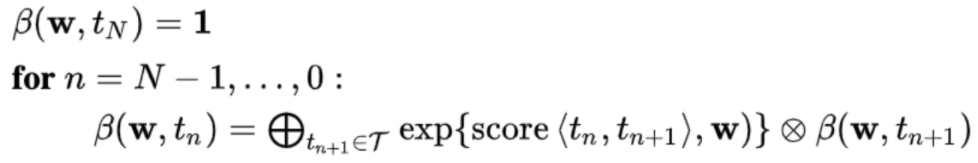
\includegraphics[width=.23\textwidth]{img/CRF-normalizer.png}
\end{center}
\vspace{-0.5cm}

\subsection*{Decoding the best POS tagging}

Find maximum-score path, using Viterbi (semiring: $([0,1], \max, \times, 0, 1)$).

\subsection*{Semiring}

Def: (1) $(A, \oplus, \bar{0})$ commutative monoid, (2) $(A, \otimes, \bar{1})$ monoid, (3) $\otimes$ distributes over $\oplus$: $\forall a,b,c\in A$, $(a \oplus b) \otimes c=(a \otimes c) \oplus(b \otimes c)$,$c \otimes(a \oplus b)=(c \otimes a) \oplus(c \otimes b)$. (4) $\bar{0}$ annohilator for $\otimes$: $\forall a \in A$, $\overline{0} \otimes a=a \otimes \overline{0}=\overline{0}$.

\vspace{-0.5cm}
\begin{center}
    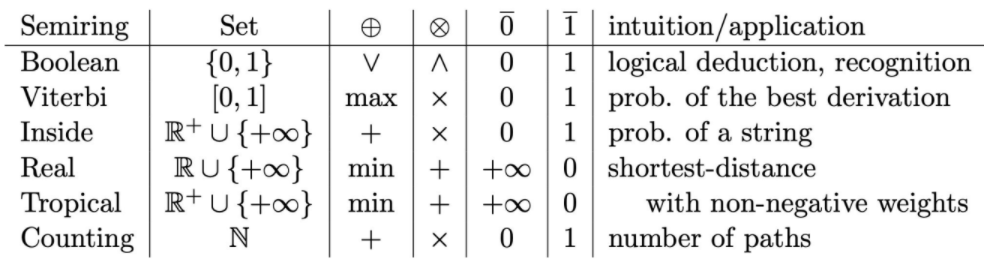
\includegraphics[width=\columnwidth]{img/semiring.png}
\end{center}
\vspace{-0.5cm}
\subsection*{Structured Perceptron}

The MLE loss for CRF is a softmax, so we add a temperature variable and take it to infinity, the loss becomes $\sum_i (\text{score}(t^i, w^i) - \max_{t^\prime} \text{score}(t^\prime, w^i))$. This is called structured perceptron.
